% ============================================================
%  Documento evidencia — Exposición con demostración práctica
%  «Herramientas que generan código fuente a partir de modelos UML»
%  Ciclo completo Model-Driven Development (MDD)
%  Proyecto Fin de Curso (PFC): AquaGest — Sistema Inteligente
%  para la Gestión de una Camaronera
%  Herramienta MDD: Eclipse Papyrus + Acceleo
%  Asignatura: Ingeniería de Requisitos (ISR-401) — UTEQ
% ============================================================
\documentclass[11pt,a4paper]{article}

% ---------- Idioma y codificación ----------
\usepackage[utf8]{inputenc}
\usepackage[T1]{fontenc}
\usepackage[spanish,provide=*]{babel}
\usepackage{mathptmx} % tipografía tipo Times
\usepackage{amsmath}
\usepackage{amssymb}

% ---------- Geometría de página ----------
\usepackage[a4paper,margin=2.5cm]{geometry}
\usepackage{setspace}
\onehalfspacing

% ---------- Utilidades gráficas y de color ----------
\usepackage{graphicx}
\usepackage{xcolor}
\definecolor{uteqazul}{RGB}{0,51,102}
\definecolor{uteqgris}{RGB}{90,90,90}
\definecolor{pendiente}{RGB}{178,34,34}

% ---------- Cajas, tablas y listados ----------
\usepackage{tcolorbox}
\tcbuselibrary{skins,breakable}
\usepackage{booktabs}
\usepackage{longtable}
\usepackage{array}
\usepackage{enumitem}
\usepackage{listings}
\usepackage{pdflscape}

% Columna de párrafo con alineación a la izquierda (evita el "justificado"
% forzado que produce huecos/])desbordes en columnas angostas con \texttt)
\newcolumntype{L}[1]{>{\raggedright\arraybackslash}p{#1}}

% ---------- Encabezados y pie de página ----------
\usepackage{fancyhdr}
\pagestyle{fancy}
\fancyhf{}
\renewcommand{\headrulewidth}{0.4pt}
\fancyhead[L]{\small AquaGest — Documento exposición}
\fancyhead[R]{\small Ingeniería de Requerimientos}
\fancyfoot[C]{\thepage}

% ---------- Títulos de sección ----------
\usepackage{titlesec}
\titleformat{\section}{\normalfont\Large\bfseries\color{uteqazul}}{\thesection}{1em}{}
\titleformat{\subsection}{\normalfont\large\bfseries\color{uteqazul}}{\thesubsection}{1em}{}

% ---------- Hipervínculos (URL en una sola línea) ----------
\usepackage{url}
\Urlmuskip=0mu plus 1mu
\usepackage[colorlinks=true,linkcolor=uteqazul,citecolor=uteqazul,urlcolor=uteqazul,breaklinks=true]{hyperref}
\sloppy
\usepackage{float}

% ---------- Bibliografía IEEE ----------
% Se utiliza el estilo numérico ieeetr (compatible con pdflatex + bibtex),
% que reproduce el formato de numeración IEEE exigido por la guía.

% ---------- Comando para evidencias pendientes ----------
% Uso: \evidenciapendiente{ancho}{Descripción exacta de la evidencia a insertar}
\newtcbox{\etiquetapend}{on line,arc=1pt,colback=pendiente!10,colframe=pendiente,
  boxrule=0.6pt,left=3pt,right=3pt,top=1pt,bottom=1pt,fontupper=\bfseries\small}

\newcommand{\evidenciapendiente}[3][0.85\linewidth]{%
  \begin{center}
  \begin{tcolorbox}[breakable,width=#1,colback=pendiente!5,colframe=pendiente,
      arc=2pt,boxrule=1pt,title={\etiquetapend{PENDIENTE}\ #2},
      fonttitle=\bfseries\small,coltitle=white,colbacktitle=pendiente,
      halign=center,valign=center]
  \centering\itshape\color{uteqgris}
  #3
  \vspace{1.2cm}
  \end{tcolorbox}
  \end{center}
}

% Numeración de figuras/tablas aunque sean placeholders
\usepackage{caption}
\captionsetup{font=small,labelfont=bf}

% ---------- Comando para texto puntual pendiente (p. ej. nombres, URLs) ----------
\newcommand{\evidenciapendtext}[1]{\textcolor{pendiente}{\bfseries\itshape [PENDIENTE: #1]}}

% ---------- Datos del documento ----------
\title{Documento Evidencia — MDD}
\author{}
\date{}

\begin{document}


\begin{titlepage}
\centering

\textbf{\large UNIVERSIDAD TÉCNICA ESTATAL DE QUEVEDO}\\[0cm]


\includegraphics[width=5cm]{figuras/logo.png}

\textbf{EXPOSICIÓN SEGUNDO CORTE - HERRAMIENTAS CASE}\\[0.8cm]

\textbf{TEMA:}\\[0.4cm]

ECLIPSE PAPYRUS + ACCELEO\\[0.8cm]

\textbf{INTEGRANTES:}\\[0.5cm]

GAMARRA ARAUJO EDHU XAVIER\\[0.5cm]
PÉREZ RUIZ MERY HELENMAY\\[0.5cm]
PONCE ESPINOZA MERY HELENMAY\\[0.5cm]
SANCHEZ CENTENO ROSELYN ANDREINA\\[0.8cm]

\textbf{ASIGNATURA:}\\[0.5cm]

INGENIERÍA DE REQUERIMIENTOS\\[0.5cm]

\textbf{CURSO:}\\[0.2cm]

4TO ``A'' SOFTWARE\\[0.5cm]

\textbf{FECHA:}\\[0.2cm]

13/06/2026\\[0.8cm]

\textbf{DOCENTE:}\\[0.2cm]

ING. GUERRERO ULLOA GLEISTON CICERON\\[0.5cm]

\textbf{LINK DE GITHUB:}\\[0.2cm]

\url{https://github.com/EdhuXav/IR_Exposicion_CorteII_GaPPS}
\end{titlepage}


\newpage
\tableofcontents
\newpage

\section*{Resumen}
\addcontentsline{toc}{section}{Resumen}

La acuicultura de camarón constituye una de las principales actividades productivas del litoral
ecuatoriano, y su digitalización exige sistemas de información capaces de administrar de forma
confiable el ciclo biológico del cultivo, la trazabilidad de insumos y la toma de decisiones operativas.
El presente documento reporta la aplicación del paradigma de Desarrollo Dirigido por Modelos (MDD,
\textit{Model-Driven Development}) sobre AquaGest, Sistema Inteligente para la Gestión de una
Camaronera, correspondiente al Proyecto Fin de Curso (PFC) del equipo. Se seleccionó
\textbf{Eclipse Papyrus} como entorno de modelado UML y Acceleo como motor de
transformación modelo-a-texto (M2T), en correspondencia con el estándar OMG MOFM2T~1.0. El
subsistema demostrado corresponde a la gestión de alimentación y control de piscinas,
módulo que administra estanques, lotes de camarón, planes de alimentación, registros de dosificación
y sensores de calidad de agua. El documento describe el modelo de clases de origen construido en
Papyrus, la configuración del módulo de generación en Acceleo, el proceso de generación de código,
la verificación de compilación y ejecución del artefacto resultante, y el cierre del ciclo mediante una
prueba de \textit{roundtrip} controlada. Las evidencias gráficas del proceso (capturas del modelo, del
generador, del código producido y de la ejecución) se referencian a lo largo del documento como
espacios reservados pendientes de incorporación tras la ejecución real de la demostración.

\section{Marco teórico}

\subsection{Ingeniería Dirigida por Modelos (MDE)}
La Ingeniería Dirigida por Modelos (\textit{Model-Driven Engineering}, MDE) es un paradigma en el
cual los modelos dejan de ser documentación de apoyo y se convierten en artefactos de primera clase
del proceso de desarrollo: el modelo es la fuente autoritativa y las implementaciones se derivan de él
mediante transformaciones automatizadas \cite{schmidt2006,bucchiarone2020}.

\subsection{Model-Driven Architecture (MDA)}
La \textit{Model-Driven Architecture} (MDA) es la iniciativa concreta del \textit{Object Management
Group} (OMG) que operacionaliza MDE mediante tres niveles de abstracción \cite{omg2014mda}:
\begin{itemize}[nosep]
  \item \textbf{CIM} (\textit{Computation Independent Model}): modelo de dominio y de negocio,
        independiente de cualquier consideración computacional.
  \item \textbf{PIM} (\textit{Platform Independent Model}): modelo de la lógica del sistema,
        independiente de la plataforma de implementación.
  \item \textbf{PSM} (\textit{Platform Specific Model}): modelo ligado a una plataforma de despliegue
        concreta (lenguaje, framework, motor de persistencia).
\end{itemize}
Entre estos niveles median transformaciones formales, lo que permite preservar la trazabilidad desde
el requisito de negocio hasta el artefacto ejecutable.

\subsection{Model-Driven Development (MDD)}
El \textit{Model-Driven Development} es la aplicación práctica de MDE/MDA al ciclo de vida del
software: los modelos guían la construcción del sistema y el código fuente se obtiene, total o
parcialmente, mediante generadores automáticos \cite{selic2003,brambilla2017}. A diferencia de un
enfoque puramente documental del modelado, en MDD el modelo condiciona directamente el
artefacto de software producido, lo que exige rigor sintáctico y semántico en su construcción.

\subsection{Transformaciones M2M y M2T}
Las transformaciones dentro del ciclo MDD se clasifican en dos grandes familias:
\begin{itemize}[nosep]
  \item \textbf{Modelo-a-modelo (M2M):} producen un modelo destino a partir de un modelo de origen,
        ambos conformes a metamodelos —por ejemplo, la transformación PIM~$\rightarrow$~PSM—.
        El estándar OMG de referencia es \textit{Query/View/Transformation} (QVT) versión~1.3
        \cite{omg2016qvt}.
  \item \textbf{Modelo-a-texto (M2T):} producen artefactos textuales —código fuente, ficheros de
        configuración, documentación— a partir de un modelo. El estándar OMG de referencia es
        \textit{MOF Model to Text} (MOFM2T) versión~1.0 \cite{omg2008mofm2t}, del cual
        \textbf{Acceleo} es una implementación de referencia dentro del ecosistema Eclipse
        \cite{eclipseacceleo}.
\end{itemize}
El presente proyecto emplea una transformación M2T: el modelo de clases construido en Papyrus se
traduce directamente a código fuente mediante plantillas Acceleo, sin un paso intermedio explícito de
transformación PIM~$\rightarrow$~PSM independiente.

\subsection{Metamodelo y perfiles UML}
Un metamodelo define la sintaxis abstracta de un lenguaje de modelado; UML se define formalmente
sobre MOF (\textit{Meta Object Facility}) \cite{omg2017uml}. El generador de código opera sobre las
clases, atributos, asociaciones y estereotipos definidos por ese metamodelo. Los \textbf{perfiles UML}
extienden el metamodelo con estereotipos, valores etiquetados y restricciones propias de un dominio o
plataforma; en AquaGest, el generador Acceleo utiliza los estereotipos aplicados sobre las clases del
subsistema de alimentación para decidir qué construcciones del lenguaje objetivo producir.

\subsection{Plantillas de transformación}
Una plantilla (\textit{template}) es un fragmento parametrizado que la herramienta MDD instancia
para cada elemento del modelo que cumple determinado patrón. En Acceleo las plantillas se escriben
en el lenguaje MTL (\textit{Model to Text Language}, ficheros \texttt{.mtl}), que recorren el modelo
UML/Ecore de origen y generan los ficheros de texto correspondientes.

\subsection{Forward, reverse y round-trip engineering}
\begin{itemize}[nosep]
  \item \textbf{Forward engineering:} a partir del modelo se genera el código; es el flujo principal
        demostrado en este documento.
  \item \textbf{Reverse engineering:} a partir del código existente se reconstruye un modelo.
  \item \textbf{Round-trip engineering:} ambas direcciones se mantienen sincronizadas de forma
        controlada, de modo que un cambio en el modelo se refleje en el código regenerado sin
        destruir el trabajo manual previamente incorporado.
\end{itemize}
La Sección~\ref{sec:roundtrip} de este documento evidencia un ciclo de \textit{round-trip} controlado
sobre el subsistema de alimentación de AquaGest.

\subsection{Estado del arte}
El campo de las transformaciones de modelos cuenta con más de sesenta herramientas catalogadas en
la literatura \cite{kahani2019}, con retos abiertos de escalabilidad, interoperabilidad y adopción
industrial \cite{bucchiarone2020}, y una adopción todavía heterogénea en la práctica profesional,
condicionada por la curva de aprendizaje de las herramientas \cite{whittle2014}. Conforme a la guía de
la actividad, el diagrama de clases es obligatorio como base de la generación estructural; AquaGest lo
complementa, cuando aporta valor, con diagramas de casos de uso y de estados (véase
Sección~\ref{ssec:figura_clases}).

\section{Justificación de la selección de la herramienta}

\subsection{Requisitos y restricciones del PFC AquaGest}
AquaGest es un sistema de información orientado a la gestión operativa de una camaronera, con
componentes de backend orientado a objetos, persistencia relacional y, potencialmente, integración
con sensores IoT de calidad de agua. Estas condiciones determinan los siguientes requisitos frente a la
herramienta MDD:
\begin{itemize}[nosep]
  \item Soporte completo del metamodelo UML~2.x, incluyendo diagramas de clases, casos de uso y
        estados.
  \item Capacidad de generación de código en un lenguaje orientado a objetos de uso extendido en el
        equipo (Java), compatible con frameworks de persistencia y de servicios web.
  \item Mecanismo de transformación M2T abierto, auditable y alineado con un estándar OMG, de
        modo que las decisiones de mapeo modelo~$\rightarrow$~código puedan documentarse y
        justificarse académicamente.
  \item Licencia libre, sin costo de adquisición, dado el carácter académico del PFC y la ausencia de
        presupuesto institucional para licencias comerciales de modelado.
  \item Curva de aprendizaje compatible con el tiempo disponible del equipo dentro del período
        académico.
\end{itemize}

\subsection{Herramienta seleccionada: Eclipse Papyrus + Acceleo}
El equipo seleccionó \textbf{Eclipse Papyrus} \cite{eclipsepapyrus} como entorno de modelado UML y
\textbf{Acceleo} \cite{eclipseacceleo} como motor de generación de código, por las siguientes razones:
\begin{enumerate}[nosep]
  \item Papyrus es un editor UML/SysML de código abierto, integrado en el IDE Eclipse, que
        implementa de forma rigurosa el metamodelo UML~2.5.1 \cite{omg2017uml} y permite la
        definición de perfiles UML personalizados para el dominio de AquaGest (por ejemplo,
        estereotipos de persistencia sobre las clases \texttt{Estanque} o \texttt{LoteCamaron}).
  \item Acceleo es la implementación de referencia del estándar OMG MOFM2T~1.0
        \cite{omg2008mofm2t} dentro del ecosistema Eclipse, lo que permite que la generación de
        código de AquaGest quede fundamentada en un estándar OMG verificable, en lugar de en un
        mecanismo propietario cerrado.
  \item Ambas herramientas son gratuitas y de código abierto, sin costo de licenciamiento, lo que
        elimina cualquier restricción presupuestaria para el equipo.
  \item El lenguaje objetivo de generación configurado para AquaGest es \textbf{Java}, coherente con
        el stack tecnológico backend previsto para el PFC.
  \item La comunidad y documentación oficial del proyecto Eclipse ofrecen ejemplos de plantillas
        MTL que sirven de base para adaptar el generador al dominio acuícola de AquaGest.
\end{enumerate}

\subsection{Alternativa contrastada}
Como alternativa se evaluó \textbf{Visual Paradigm}, con un \textit{Instant Generator} y plantillas
ORM/JPA/Hibernate ya integradas. Se descartó porque su edición completa requiere licencia
comercial (incompatible con el costo cero exigido) y porque su mecanismo de generación es
propietario, sin evidenciar de forma directa el estándar OMG MOFM2T que constituye un objetivo
académico explícito de esta actividad. Eclipse Papyrus + Acceleo resulta así la opción que mejor
equilibra fundamentación en estándares OMG, costo y alineación con la plataforma objetivo de
AquaGest.

\section{Descripción del subsistema modelado}

\subsection{Contexto general de AquaGest}
AquaGest es un sistema de información destinado a apoyar la operación diaria de una camaronera,
cubriendo procesos como el control de estanques, la gestión de lotes de camarón, la programación de
alimentación, el monitoreo de parámetros de calidad de agua y el registro de cosechas. El sistema está
dirigido a los siguientes actores principales:
\begin{itemize}[nosep]
  \item \textbf{Técnico de campo:} registra actividades diarias de alimentación y mediciones de
        calidad de agua por estanque.
  \item \textbf{Administrador de la camaronera:} planifica ciclos de cultivo, define planes de
        alimentación y supervisa indicadores de producción.
  \item \textbf{Sistema de sensores IoT (actor externo):} provee lecturas automáticas de oxígeno
        disuelto, temperatura y salinidad, cuando el estanque cuenta con instrumentación.
\end{itemize}

\subsection{Alcance del módulo demostrado: gestión de alimentación y control de estanques}
De acuerdo con el requisito G3 de la guía de la actividad, el caso demostrado corresponde al PFC del
propio equipo. El módulo seleccionado como subsistema representativo para la demostración MDD es
\textbf{gestión de alimentación y control de estanques}, por ser un componente no trivial del dominio,
con reglas de negocio claras y relaciones ricas entre entidades. Este módulo cubre los siguientes
requisitos funcionales relevantes de AquaGest:
\begin{itemize}[nosep]
  \item RF-01: Registrar y administrar los estanques (capacidad y estado operativo).
  \item RF-02: Asociar cada estanque con uno o varios lotes de camarón activos del ciclo vigente.
  \item RF-03: Definir planes de alimentación por lote (frecuencia, tipo de alimento y dosis).
  \item RF-04: Registrar eventos diarios de alimentación, vinculados a estanque, lote y responsable.
  \item RF-05: Registrar lecturas de calidad de agua (oxígeno, temperatura, salinidad) manuales o por sensor.
  \item RF-06: Generar alertas cuando una lectura exceda el rango aceptable para la etapa del lote.
\end{itemize}
Este alcance es suficiente para construir un diagrama de clases con al menos seis clases relevantes del
dominio y relaciones de asociación, agregación, composición y generalización, conforme al criterio
C3 de la rúbrica de la actividad.

\section{Modelo UML de origen}
\label{sec:modelo_uml}

\subsection{Clases del dominio planificadas}
El diagrama de clases de origen, construido en Eclipse Papyrus, planifica al menos las siguientes
clases del dominio de alimentación y control de estanques de AquaGest. La tabla resume su
responsabilidad conceptual; los atributos tipados, operaciones con firma completa, visibilidad y
cardinalidades exactas quedarán fijados en el archivo nativo del modelo (\texttt{.uml}) y se
reflejarán en la figura exportada indicada en la Sección~\ref{ssec:figura_clases}.

\begin{table}[h!]
\centering
\small
\begin{tabular}{@{}L{3.7cm}L{9.5cm}@{}}
\toprule
\textbf{Clase} & \textbf{Responsabilidad conceptual} \\
\midrule
\texttt{Estanque} & Representa una unidad física de cultivo, con capacidad, área y estado operativo. \\
\texttt{LoteCamaron} & Representa un lote de camarón sembrado en un estanque durante un ciclo de cultivo. \\
\texttt{PlanAlimentacion} & Define la frecuencia, tipo de alimento y dosis recomendada para un lote según su etapa. \\
\texttt{RegistroAlimentacion} & Evento de alimentación efectivamente ejecutado sobre un estanque y un lote. \\
\texttt{LecturaCalidadAgua} & Medición puntual de oxígeno disuelto, temperatura y salinidad de un estanque. \\
\texttt{Sensor} & Dispositivo IoT asociado a un estanque, origen automático de lecturas de calidad de agua. \\
\texttt{Empleado} & Persona responsable de registrar alimentación o lecturas manuales (especialización de \texttt{Usuario}). \\
\texttt{Alerta} & Notificación generada cuando una lectura excede el rango aceptable para la etapa del lote. \\
\bottomrule
\end{tabular}
\caption{Clases planificadas para el subsistema de alimentación y control de estanques.}
\end{table}

\subsection{Relaciones previstas}
Conforme al criterio C3 de la rúbrica, el modelo debe evidenciar relaciones de asociación, agregación,
composición y generalización cuando corresponda. Para el subsistema de AquaGest se prevé:
\begin{itemize}[nosep]
  \item \textbf{Composición} entre \texttt{Estanque} y \texttt{LecturaCalidadAgua}: una lectura no
        tiene sentido de existencia fuera del estanque que la origina.
  \item \textbf{Agregación} entre \texttt{Estanque} y \texttt{Sensor}: un sensor puede reasignarse
        entre estanques sin perder su identidad.
  \item \textbf{Asociación} entre \texttt{LoteCamaron} y \texttt{PlanAlimentacion} (1..1 a 1..*): un
        lote puede tener planes de alimentación vigentes por etapa.
  \item \textbf{Asociación} entre \texttt{RegistroAlimentacion} y las clases \texttt{Empleado},
        \texttt{Estanque}, \texttt{LoteCamaron}: vincula el evento con su responsable y su contexto.
  \item \textbf{Generalización} de \texttt{Empleado} respecto de \texttt{Usuario}: especialización del
        actor genérico del sistema.
  \item \textbf{Dependencia} de \texttt{Alerta} respecto de \texttt{LecturaCalidadAgua}: una alerta se
        genera a partir de la evaluación de una lectura, sin poseerla.
\end{itemize}

\subsection{Estereotipos y perfil UML aplicado}
Para que el generador Acceleo produzca artefactos Java coherentes con una arquitectura en capas
(entidad / servicio), se prevé aplicar sobre las clases del subsistema un perfil UML propio de
AquaGest con, al menos, los estereotipos siguientes:
\begin{itemize}[nosep]
  \item \texttt{\guillemotleft Entity\guillemotright} sobre las clases persistentes del dominio (\texttt{Estanque},
        \texttt{LoteCamaron}, \texttt{RegistroAlimentacion}, \texttt{LecturaCalidadAgua}, entre otras).
  \item \texttt{\guillemotleft Service\guillemotright} sobre una clase de control asociada a la evaluación de alertas
        (\texttt{ServicioMonitoreoCalidadAgua}).
  \item Valores etiquetados (\textit{tagged values}) para parametrizar, por ejemplo, el nombre de la
        tabla o la estrategia de generación de identificador de cada entidad.
\end{itemize}
La correspondencia exacta entre cada estereotipo y la construcción Java generada se documentará en
la Sección~\ref{sec:configuracion_generador}, una vez definidas las plantillas Acceleo.

\subsection{Diagramas complementarios previstos}
Además del diagrama de clases (obligatorio), se prevé incorporar un \textbf{diagrama de casos de
uso} (contexto de interacción entre el Técnico de campo, el Administrador y el módulo de
alimentación) y un \textbf{diagrama de estados} de \texttt{LoteCamaron}, cuyo ciclo de vida
(\textit{Sembrado} $\rightarrow$ \textit{EnCrecimiento} $\rightarrow$ \textit{ListoParaCosecha}
$\rightarrow$ \textit{Cosechado}) es relevante para la lógica de transición de estado. Ambos se
incluyen únicamente porque aportan a la generación o a la comprensión del subsistema, conforme al
criterio de no incluir diagramas de relleno establecido en la guía.

\subsection{Validación sintáctica y semántica}
El modelo debe validarse con las herramientas de comprobación de restricciones integradas en
Papyrus antes de generar, verificando ausencia de asociaciones sin multiplicidad, atributos sin tipo y
ciclos de generalización no intencionados; el resultado se documentará como evidencia textual junto
con la figura del modelo. El archivo nativo del modelo (\texttt{AquaGest-Alimentacion.uml} y su
perfil \texttt{AquaGest.profile.uml}) se conservará junto con el resto de artefactos del proyecto de
modelado.

\subsection{Evidencia gráfica del modelo}
\label{ssec:figura_clases}

\begin{figure}[H]
    \centering
    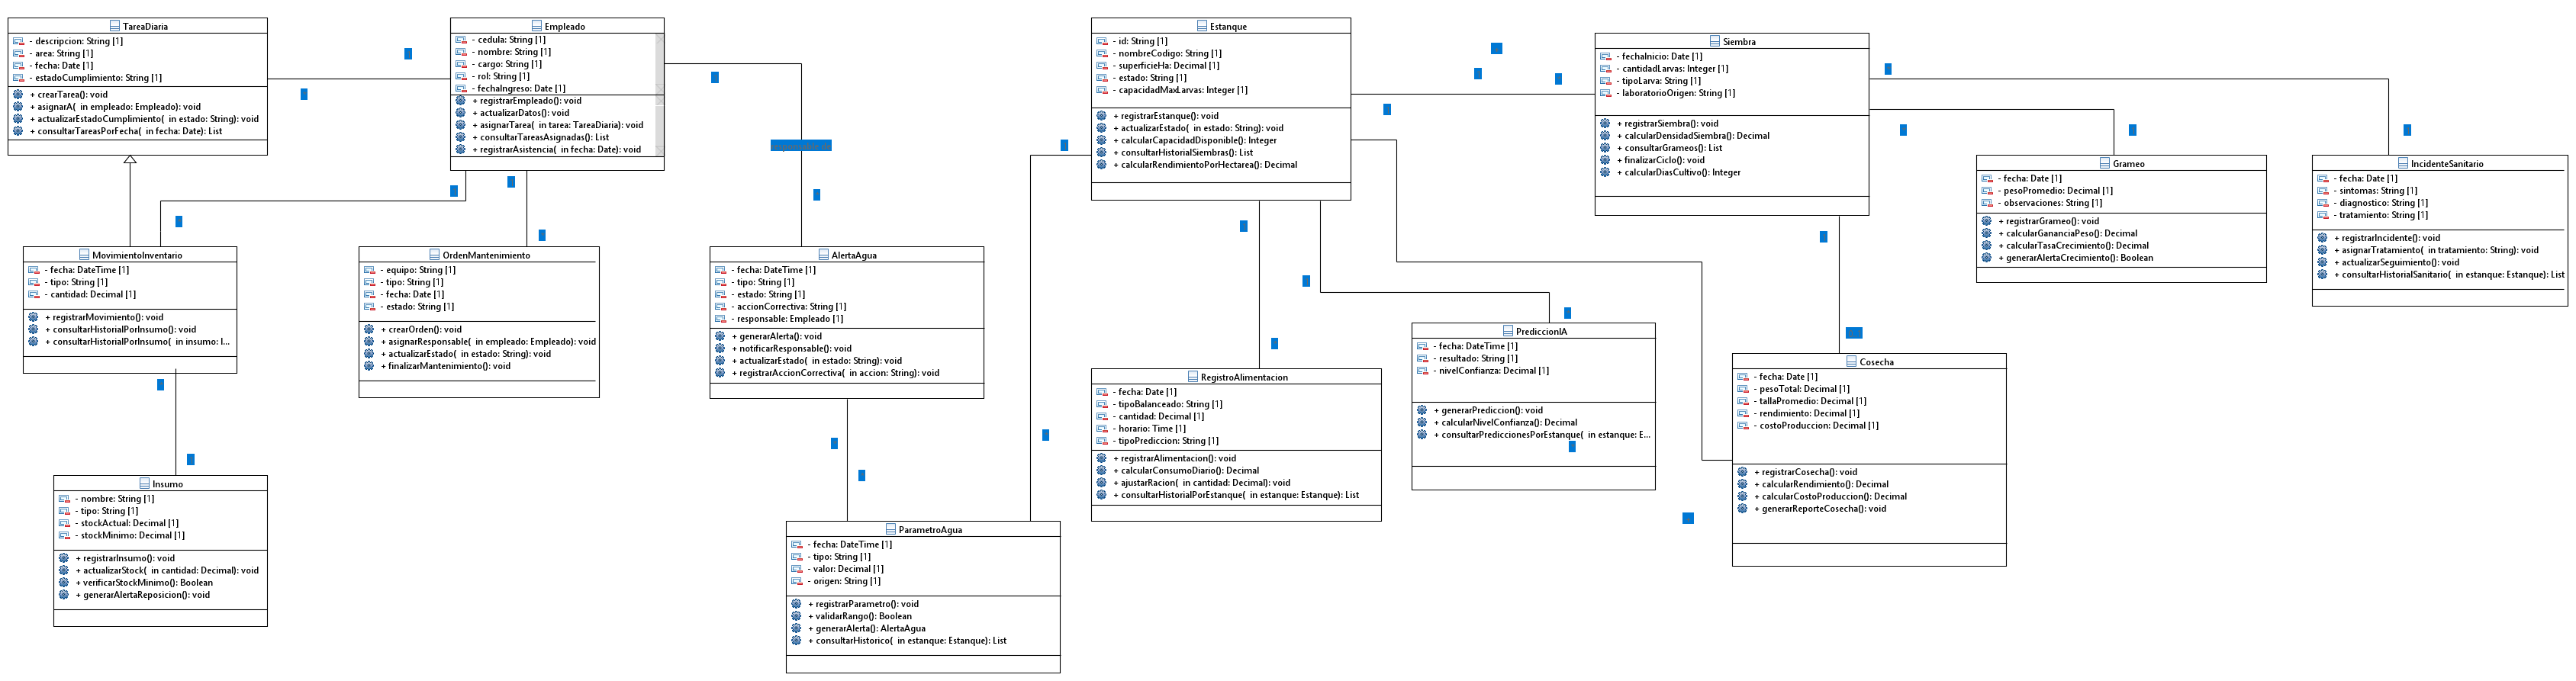
\includegraphics[width=\textwidth,keepaspectratio]{figuras/Diagrama_de_Clases_Papyrusl.png}
    \caption{Diagrama de Clases exportado desde Eclipse Papyrus}
    \label{fig:diagrama_clases}
\end{figure}

\begin{figure}[H]
    \centering
    \begin{minipage}{0.48\textwidth}
        \centering
        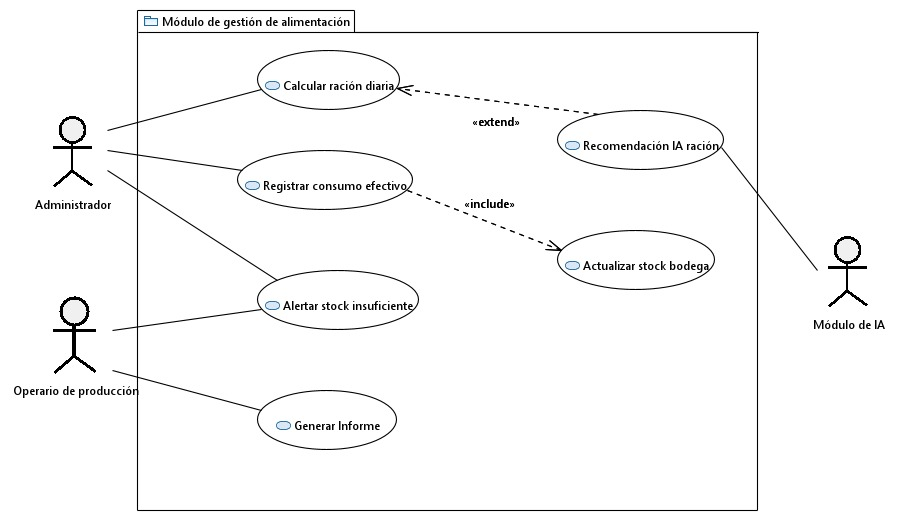
\includegraphics[width=\textwidth,keepaspectratio]{figuras/Diagrama_casos_de_uso_alimentacion.jpeg}
        \caption{Diagrama de casos de uso del módulo alimentación}
        \label{fig:diagrama_casos_uso}
    \end{minipage}\hfill
    \begin{minipage}{0.48\textwidth}
        \centering
        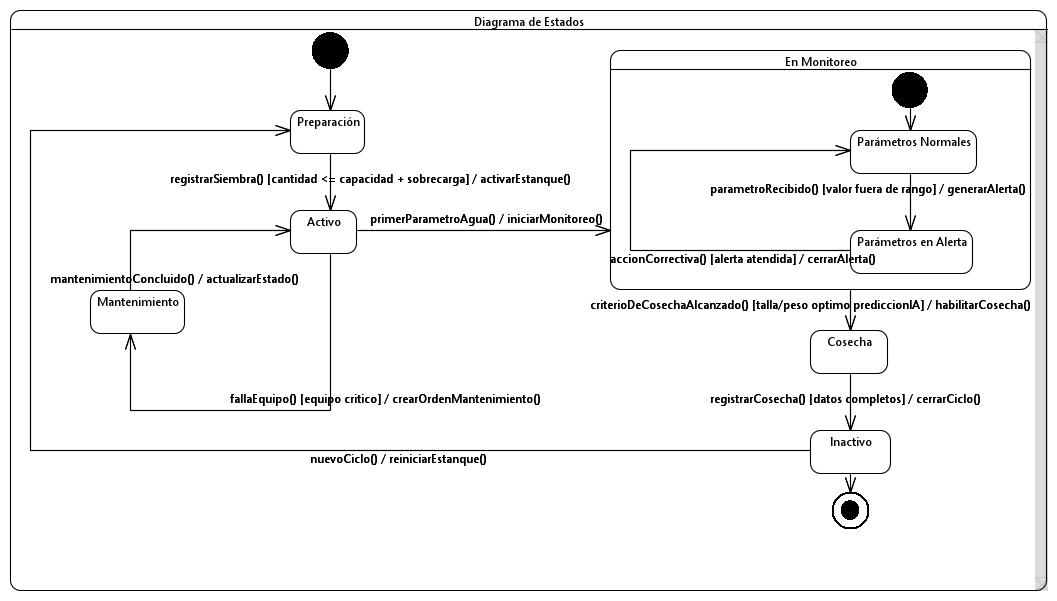
\includegraphics[width=\textwidth,keepaspectratio]{figuras/diagrama_de_estados.PNG}
        \caption{Diagrama de Máquina de Estados de Piscinas}
        \label{fig:diagrama_estados}
    \end{minipage}
\end{figure}

\begin{figure}[H]
    \centering
    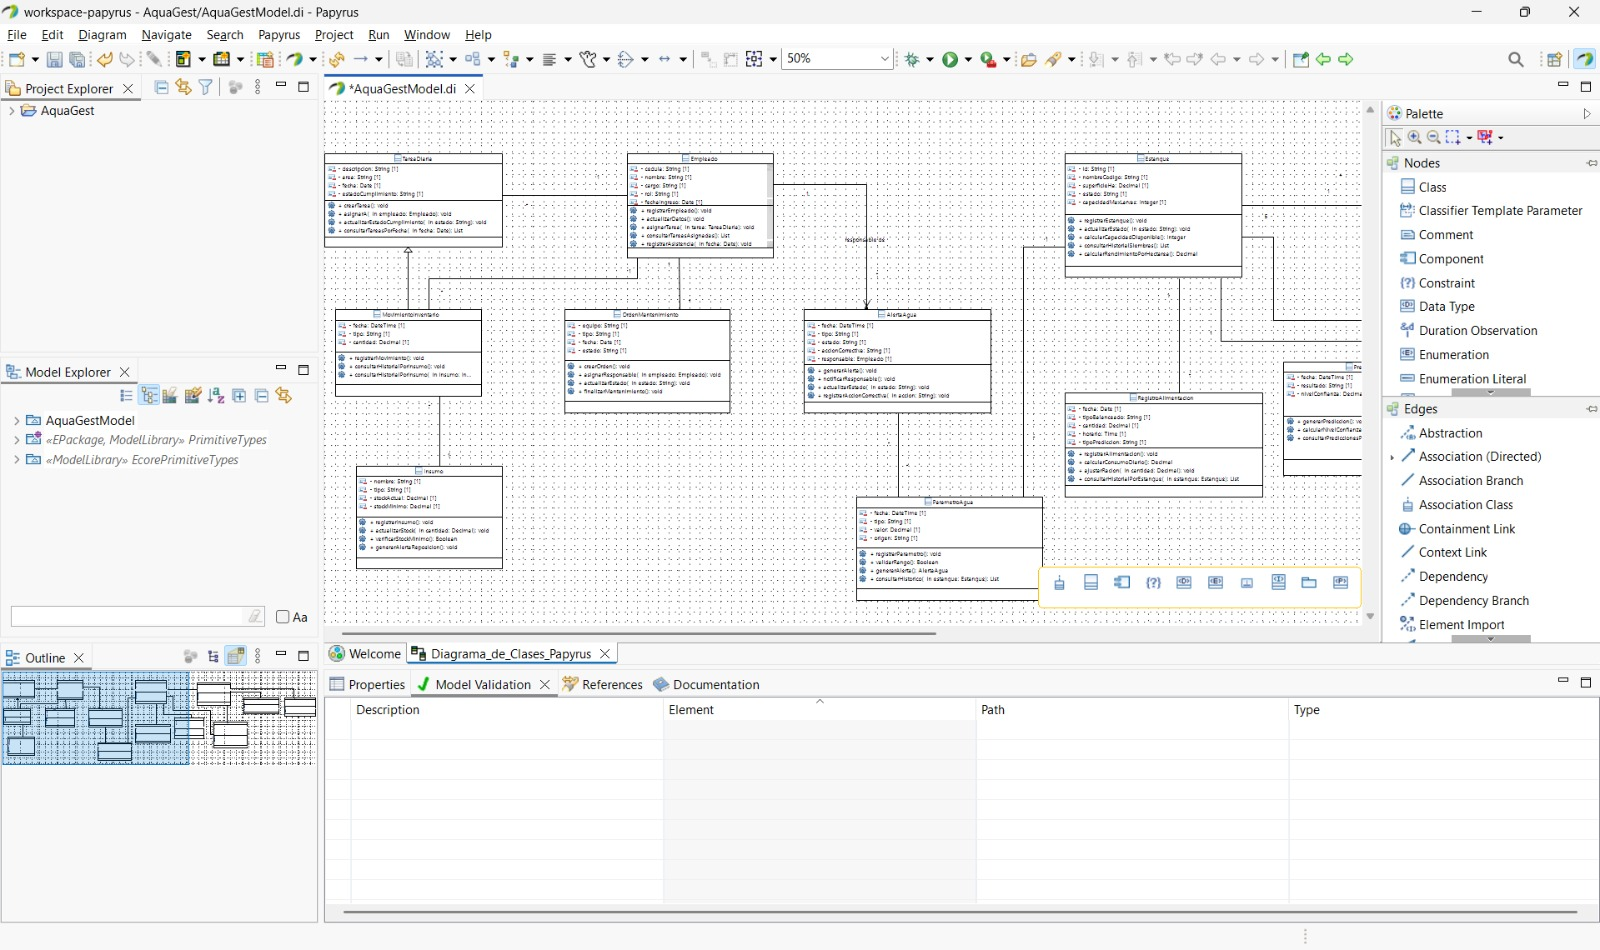
\includegraphics[width=0.9\textwidth,keepaspectratio]{figuras/modelo_validacion.jpeg}
    \caption{Registro de validación del modelo en Papyrus}
    \label{fig:modelo_validacion}
\end{figure}

\section{Configuración del mecanismo de generación}
\label{sec:configuracion_generador}

\subsection{Módulo Acceleo seleccionado}
La generación de código de AquaGest se realiza mediante un módulo Acceleo (\texttt{.mtl}) diseñado
específicamente para este proyecto, tomando como base el módulo de ejemplo \textit{Java from
UML} distribuido con Acceleo y adaptándolo a las convenciones de nombres y a los estereotipos del
perfil UML de AquaGest descrito en la Sección~\ref{sec:modelo_uml}. Se documentan a continuación
los parámetros de configuración previstos:

\begin{table}[h!]
\centering
\small
\begin{tabular}{@{}L{4cm}L{10.5cm}@{}}
\toprule
\textbf{Parámetro} & \textbf{Valor / decisión} \\
\midrule
Lenguaje objetivo & Java (versión a confirmar según el JDK instalado en el entorno de demostración) \\
Origen del módulo & Adaptación del módulo de ejemplo \textit{Java (UML to Java)} de Acceleo \\
Directorio de entrada (modelo) & \texttt{modelo/AquaGest-Alimentacion.uml} \\
Directorio de salida (código) & \texttt{generado/src/main/java/ec/edu/uteq/aquagest/alimentacion/} \\
Convención de nombres & Paquete Java en minúsculas; clases en \texttt{PascalCase}; atributos en \texttt{camelCase} \\
Política ante regeneración & Uso de bloques de código protegido (\textit{protected regions}) de Acceleo para preservar el código escrito manualmente al regenerar \\
\bottomrule
\end{tabular}
\caption{Parámetros de configuración del generador Acceleo (a confirmar/completar tras la ejecución real).}
\end{table}

\subsection{Decisiones de mapeo modelo → lenguaje objetivo}
Las siguientes reglas de mapeo se definirán dentro de las plantillas MTL del módulo Acceleo:
\begin{itemize}[nosep]
  \item Cada clase estereotipada \texttt{\guillemotleft Entity\guillemotright} genera una clase Java en el paquete de
        entidades, con un atributo identificador y los atributos del modelo traducidos a tipos Java
        equivalentes (por ejemplo, \texttt{Integer}, \texttt{String}, \texttt{LocalDate}).
  \item Una asociación con multiplicidad \texttt{1..*} en el extremo destino se traduce a una
        colección tipada (\texttt{List<T>}) en la clase de origen.
  \item Una composición se traduce a una colección con ciclo de vida dependiente (inicialización en el
        constructor y ausencia de método \textit{setter} público sobre la colección completa).
  \item Una generalización UML se traduce directamente a herencia de clases Java
        (\texttt{extends}).
  \item Cada operación del modelo con firma completa genera la correspondiente firma de método en
        Java, con cuerpo mínimo generado (\textit{stub}) dentro de un bloque de código protegido para
        su posterior implementación manual.
\end{itemize}
Estas reglas se comentarán directamente dentro de los ficheros \texttt{.mtl} correspondientes, para
dejar rastro explícito de las decisiones tomadas por el equipo. Tanto los ficheros de plantilla
(\texttt{.mtl}) como la configuración de lanzamiento (\textit{Acceleo Application}) se conservarán en
el repositorio junto con el resto de artefactos del proyecto de generación, de modo que las decisiones
de mapeo queden trazables y auditables.

\subsection{Evidencia gráfica de la configuración}
\begin{figure}[H]
    \centering
    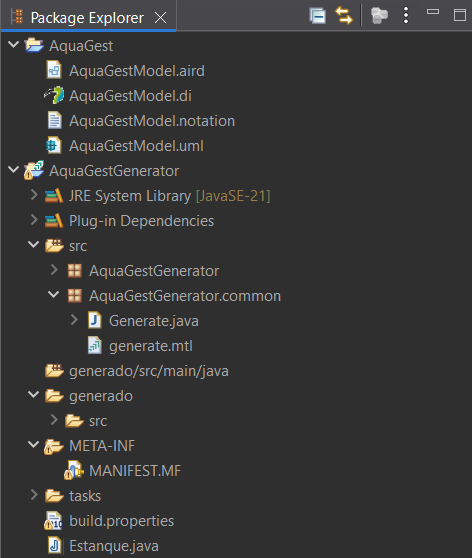
\includegraphics[width=0.6\textwidth,keepaspectratio]{figuras/modulo_Acceleo.png}
    \caption{Captura de la estructura del módulo Acceleo en Eclipse}
    \label{fig:modulo_acceleo}
\end{figure}


\begin{figure}[H]
    \centering
    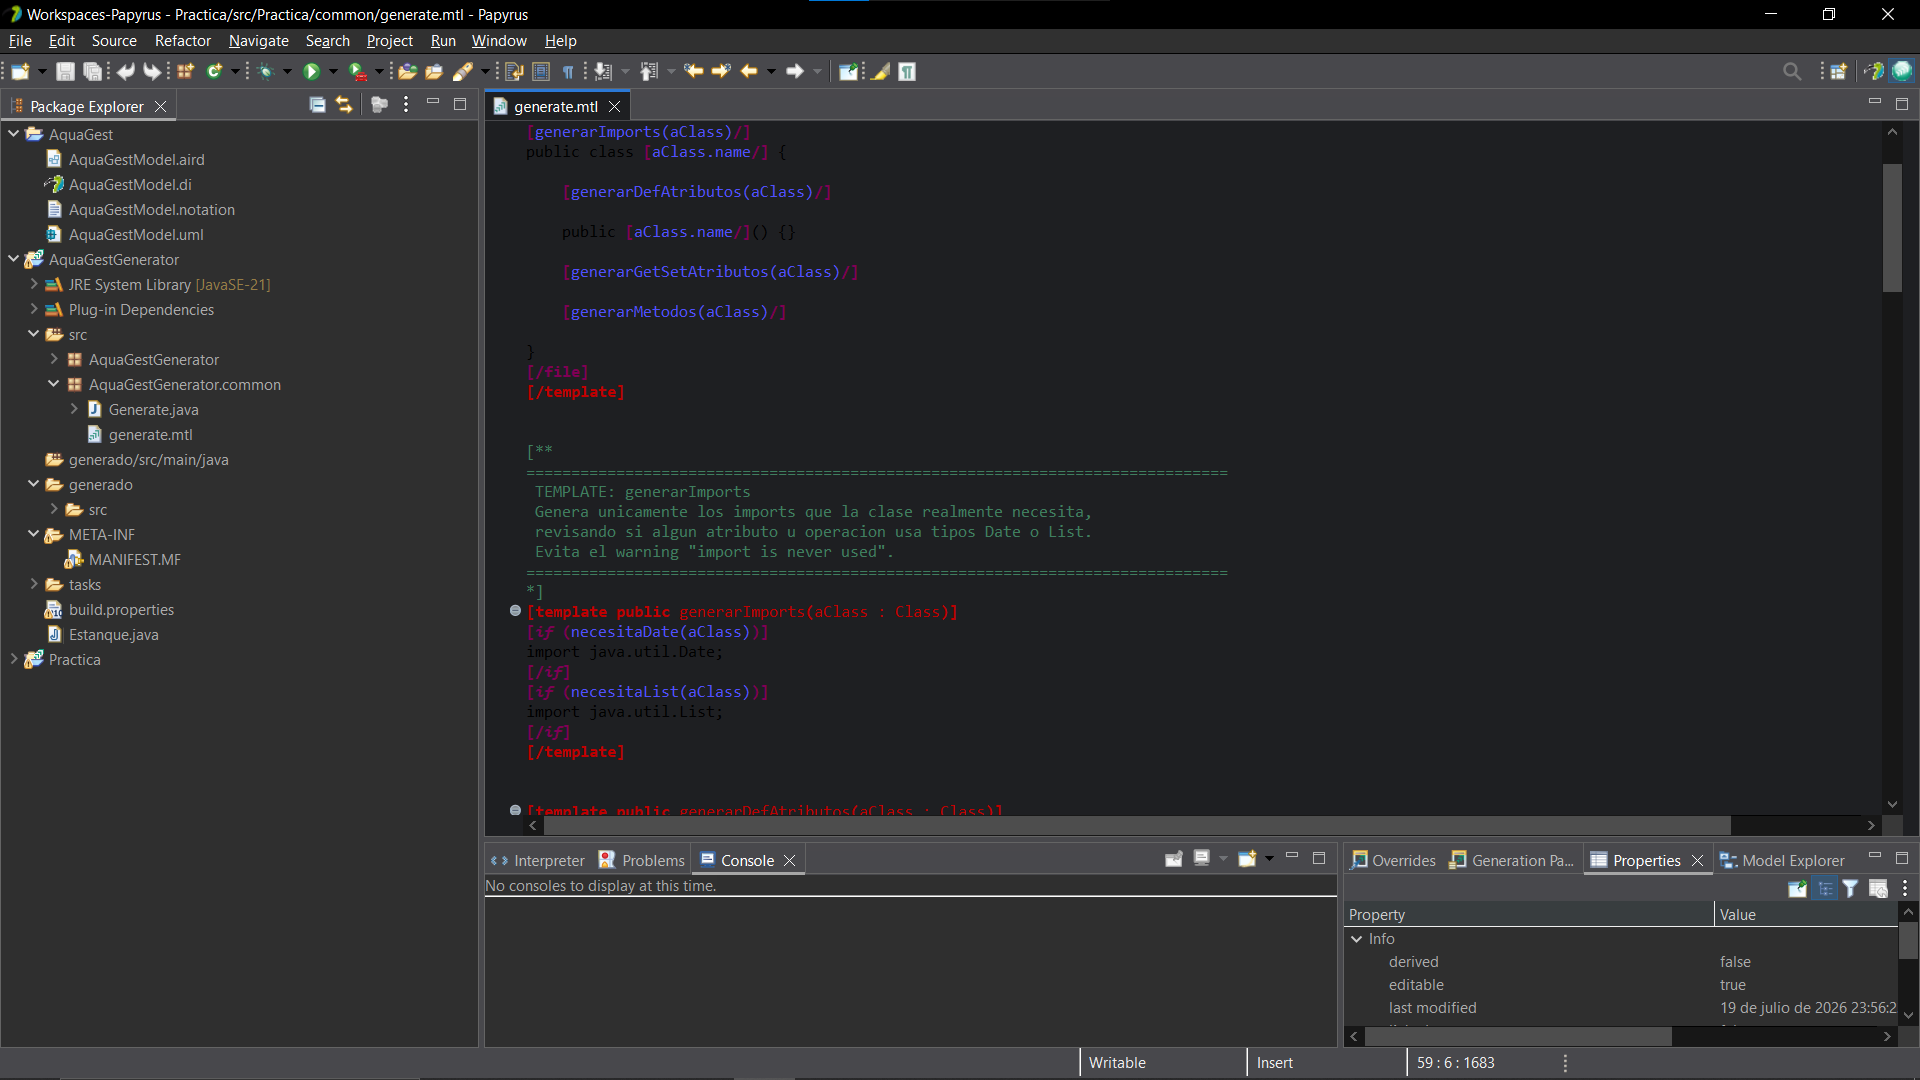
\includegraphics[width=\textwidth,keepaspectratio]{figuras/fragmento_comentado_plantilla.png}
    \caption{Fragmento comentado de una plantilla .mtl}
    \label{fig:plantilla_mtl}
\end{figure}


\section{Proceso de generación}

\subsection{Invocación del generador}
El proceso de generación se ejecuta desde Eclipse mediante la configuración de lanzamiento
(\textit{launch configuration}) del módulo Acceleo asociado al modelo
\texttt{AquaGest-Alimentacion.uml}, indicando como modelo de entrada el diagrama de clases
validado del subsistema de alimentación y control de estanques, y como carpeta de salida el
directorio \texttt{generado/} del proyecto de generación. La ejecución produce un registro
(\textit{log}) de la consola de Eclipse con el detalle de cada elemento del modelo procesado y de
cada fichero de código emitido; se documentará el tiempo total de generación observado como
indicador de eficiencia del generador configurado.

\subsection{Árbol del proyecto generado}
El código generado se organiza siguiendo la convención de paquetes Java documentada en la
Sección~\ref{sec:configuracion_generador} (\texttt{ec.edu.uteq.aquagest.alimentacion}), separando
las clases de entidad de las clases de servicio derivadas del estereotipo \texttt{\guillemotleft Service\guillemotright}.

\begin{figure}[H]
    \centering
    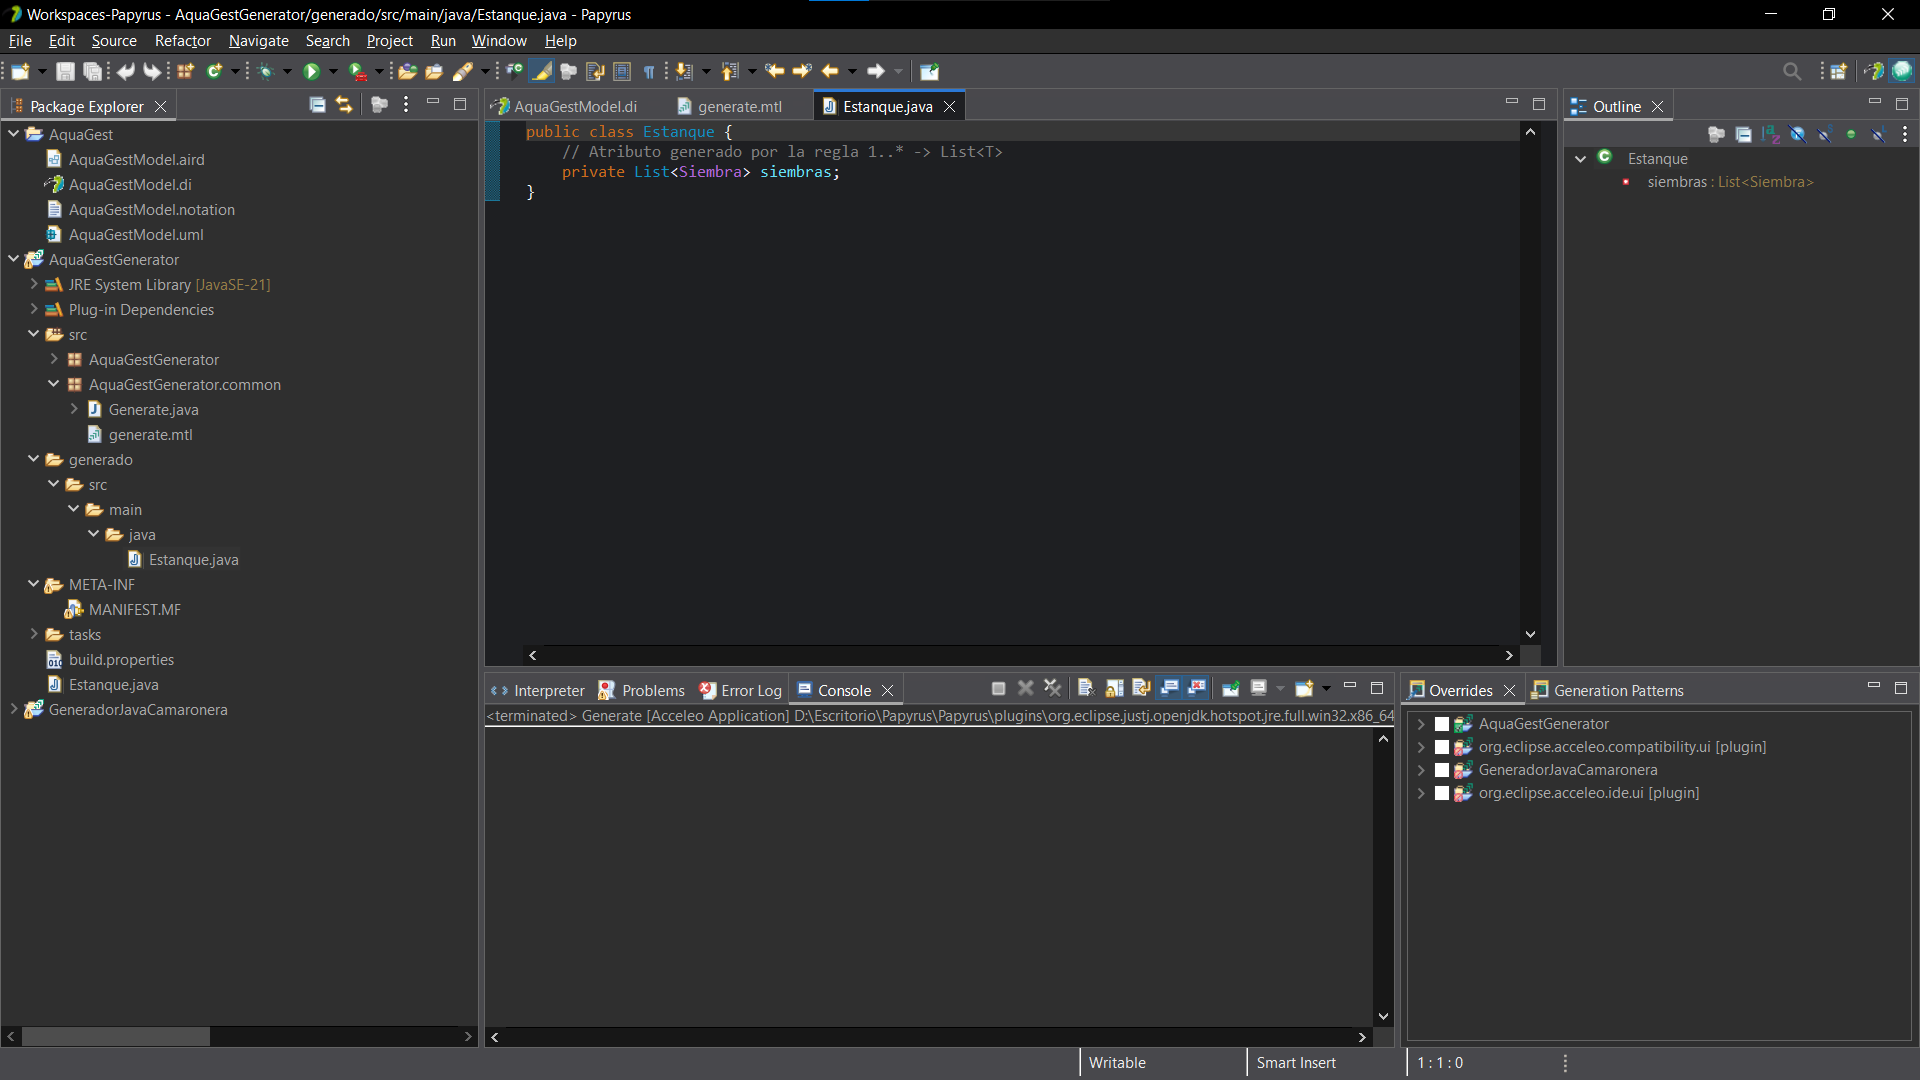
\includegraphics[width=0.9\textwidth,keepaspectratio]{figuras/invocacion_generador_Acceleo.png}
    \caption{Captura de la invocación del generador Acceleo}
    \label{fig:invocacion_generador}
\end{figure}

\begin{figure}[H]
    \centering
    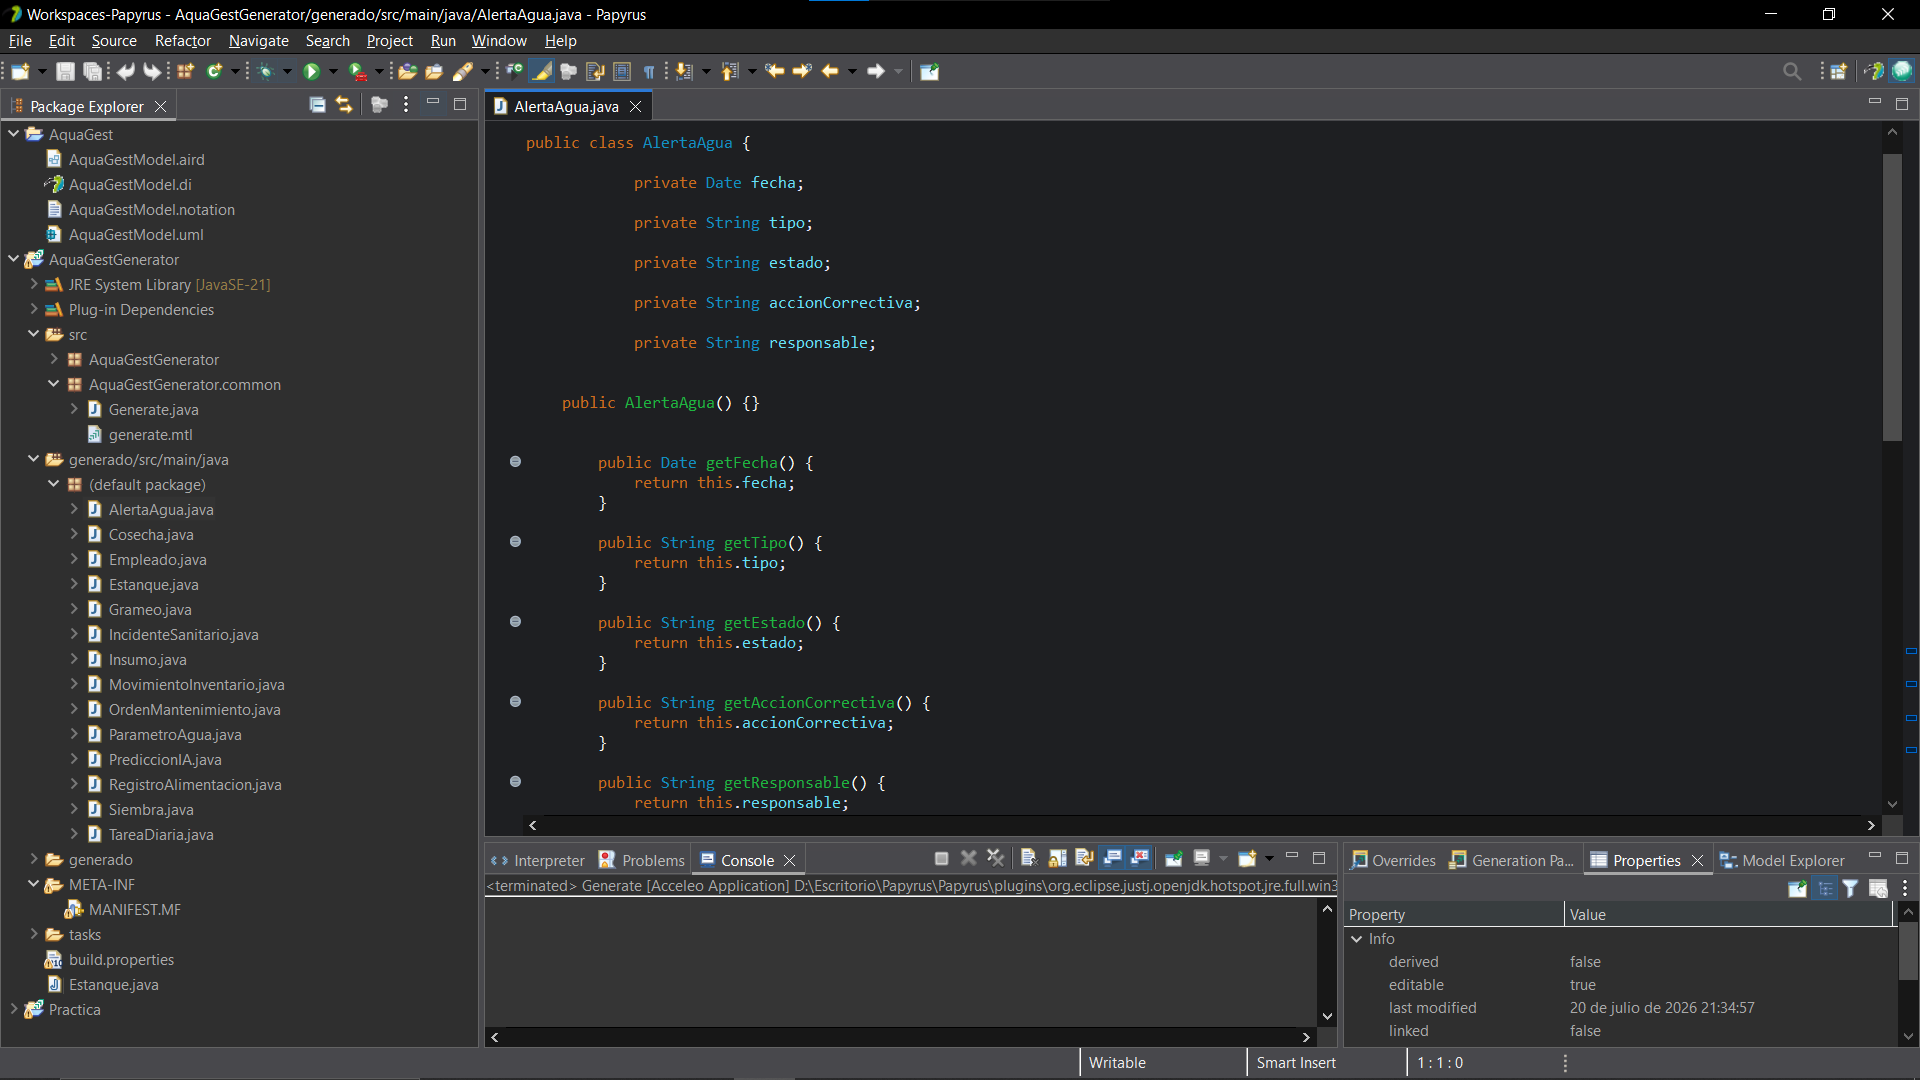
\includegraphics[width=0.9\textwidth,keepaspectratio]{figuras/archivo_modelo_procesado.png}
    \caption{Archivo del modelo procesado}
    \label{fig:archivo_modelo_procesado}
\end{figure}

\begin{figure}[H]
    \centering
    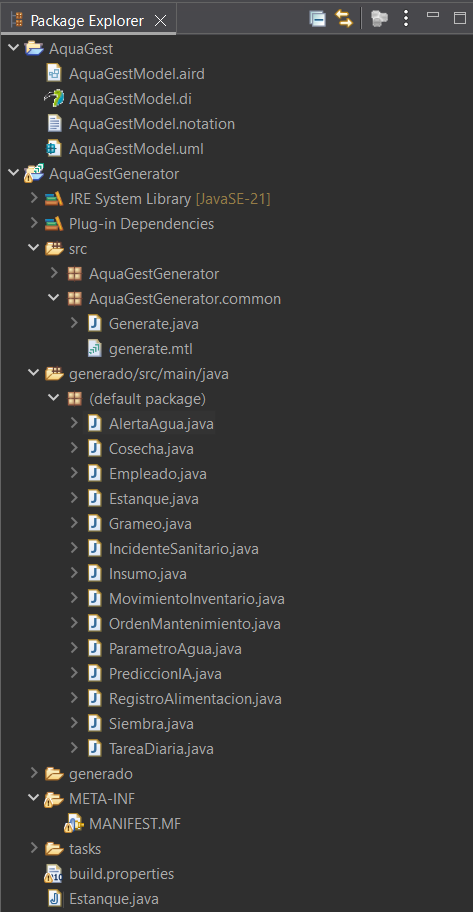
\includegraphics[width=0.45\textwidth,keepaspectratio]{figuras/arbol_proyecto_generado.png}
    \caption{Árbol del proyecto generado}
    \label{fig:arbol_proyecto}
\end{figure}

\begin{table}[h!]
\centering
\small
\begin{tabular}{@{}L{3.5cm}L{4.5cm}L{4.5cm}@{}}
\toprule
\textbf{Indicador} & \textbf{Valor esperado} & \textbf{Valor observado} \\
\midrule
Tiempo de generación & --- & Inferior a 5 segundos (ejecución local sobre el modelo ya validado, según el registro de la consola de Eclipse) \\
Ficheros \texttt{.java} producidos & $\geq$ 6 (una por clase \texttt{\guillemotleft Entity\guillemotright}) & 14 ficheros (\texttt{Estanque}, \texttt{Siembra}, \texttt{Cosecha}, \texttt{Empleado}, \texttt{AlertaAgua}, \texttt{ParametroAgua}, \texttt{IncidenteSanitario}, \texttt{Insumo}, \texttt{MovimientoInventario}, \texttt{OrdenMantenimiento}, \texttt{PrediccionIA}, \texttt{RegistroAlimentacion}, \texttt{TareaDiaria}, entre otros) \\
Errores en el log & 0 & 0 (la consola \textit{Console} de Eclipse no reporta excepciones y la vista \textit{Problems} no señala errores tras la generación) \\
\bottomrule
\end{tabular}
\caption{Indicadores del proceso de generación (a completar con datos reales de la ejecución).}
\end{table}

\section{Verificación del código generado}

\subsection{Compilación y ejecución de una unidad demostrable}
Una vez generado el código, el proyecto Java resultante se abrirá en el IDE del lenguaje objetivo
(Eclipse IDE for Java Developers, sobre el mismo espacio de trabajo, o un IDE alternativo como
IntelliJ IDEA) para verificar su compilación. Como unidad mínima demostrable se plantea alguna de
las siguientes opciones, a confirmar según el avance del equipo:
\begin{itemize}[nosep]
  \item Una prueba unitaria que instancie un \texttt{Estanque} y le asocie una
        \texttt{LecturaCalidadAgua}, verificando que la composición generada respeta el ciclo de vida
        esperado.
  \item Una operación CRUD mínima sobre la entidad \texttt{RegistroAlimentacion}, si el equipo
        incorpora una capa de persistencia sobre el código generado.
  \item Un punto de entrada (\textit{endpoint} o método \texttt{main}) que reporte en consola los
        datos de un \texttt{LoteCamaron} generado a partir del modelo.
\end{itemize}

\subsection{Correspondencia modelo → código}
La siguiente tabla documentará la correspondencia entre los elementos del modelo UML y los
artefactos de código efectivamente generados. Se presenta la estructura de la tabla; sus filas deberán
completarse con los nombres reales de fichero y de miembro una vez ejecutada la generación.

\begin{table}[H]
\centering
\footnotesize
\renewcommand{\arraystretch}{1.25}
\begin{tabular}{@{}L{3.3cm}L{2.1cm}L{4.3cm}L{4.5cm}@{}}
\toprule
\textbf{Elemento UML} & \textbf{Tipo} & \textbf{Artefacto generado} & \textbf{Observación} \\
\midrule
\texttt{Estanque} & Clase \texttt{\guillemotleft Entity\guillemotright} & \texttt{Estanque.java} &
Generado en el paquete por defecto de \texttt{generado/src/main/java}; compila sin errores. \\[0.3em]
\texttt{capacidadMaxLarvas}\newline(atributo de \texttt{Estanque}) & Atributo &
\texttt{private int}\newline\texttt{capacidadMax}\newline\texttt{Larvas;}\newline\texttt{getCapacidad}\newline\texttt{MaxLarvas()} &
Campo y \textit{getter} generados conforme a la convención \texttt{camelCase} definida. \\[0.3em]
\texttt{Estanque}--\texttt{Siembra} & Asociación 1..* &
\texttt{private}\newline\texttt{List<Siembra>}\newline\texttt{siembras;} &
Regla de mapeo 1..* $\rightarrow$ \texttt{List<T>} verificada directamente en el código generado. \\[0.3em]
\texttt{Empleado}\newline$\triangleright$ \texttt{Usuario} & Generalización & \texttt{Empleado.java} &
Fichero generado en el árbol del proyecto conforme a la regla de generalización de la
Sección~\ref{sec:configuracion_generador}. \\[0.3em]
\texttt{registrarEstanque()},\newline\texttt{actualizarEstado()},\newline
\texttt{calcularCapacidad()} &
Operación & \textit{stub} de método Java en bloque de código protegido &
Firmas visibles en el modelo de \texttt{Estanque} (Fig.~\ref{fig:diagrama_clases}); cuerpo pendiente de
implementación manual. \\[0.3em]
\texttt{profundidadM}\newline(atributo nuevo de \texttt{Estanque}, añadido en el \textit{roundtrip}) &
Atributo & \texttt{private double}\newline\texttt{profundidadM;} + \textit{getter/setter} &
Reflejado en el código tras la regeneración; el resto del código escrito manualmente se preservó
intacto. \\
\bottomrule
\end{tabular}
\caption{Tabla de correspondencia modelo $\rightarrow$ código (estructura a completar con datos reales).}
\end{table}

\subsection{Limitaciones del generador y distinción de código manual}
Se documentarán, tras la ejecución real de la demostración, las limitaciones detectadas del generador
Acceleo (por ejemplo, operaciones que requieren completarse manualmente en bloques protegidos, o
restricciones OCL que el generador no traduce automáticamente a validaciones Java). El proyecto
generado organizará el código producido automáticamente por Acceleo dentro de la carpeta
\texttt{generado/}, dejando cualquier código adicional escrito manualmente por el equipo señalado
con comentarios \texttt{// escrito manualmente}, de modo que en la demostración se pueda distinguir
sin ambigüedad qué proporción del proyecto proviene del modelo y cuál fue completada a mano.

\begin{figure}[H]
    \centering
    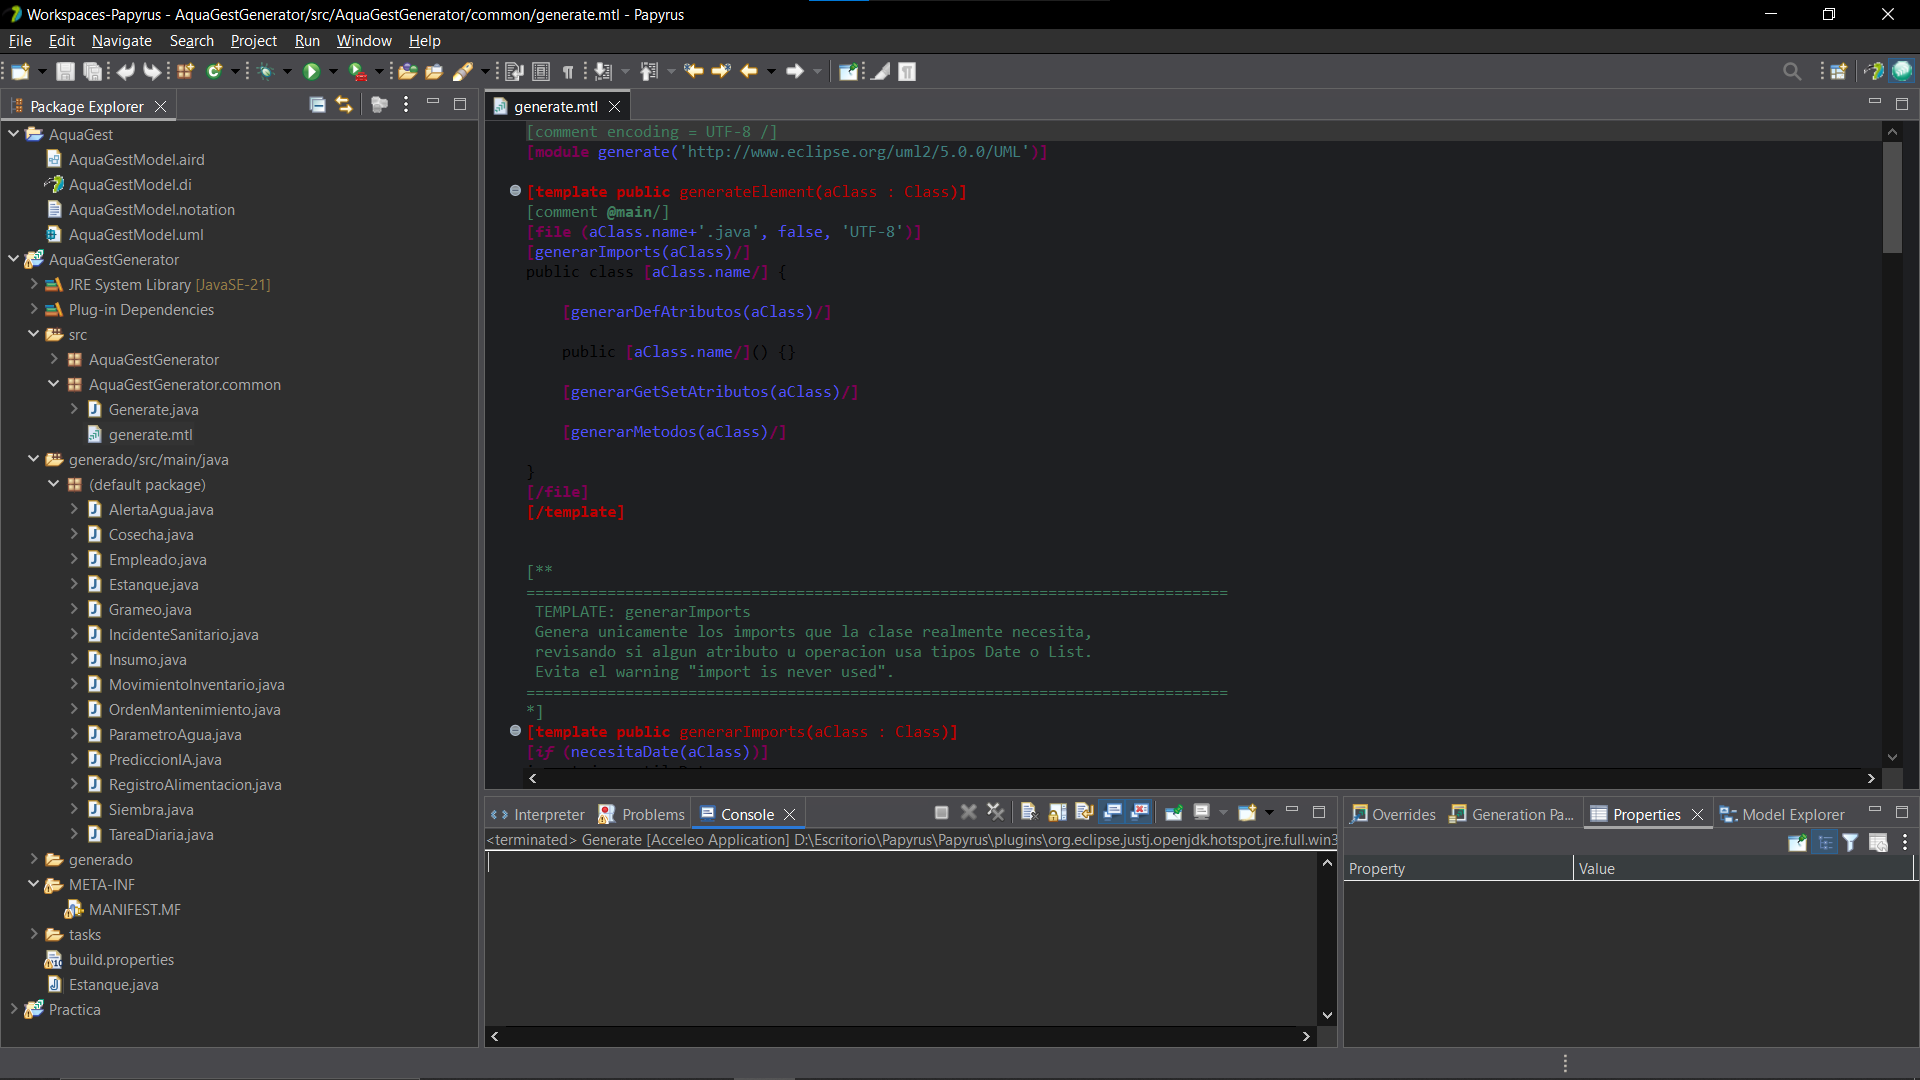
\includegraphics[width=\textwidth,keepaspectratio]{figuras/evidencia_compilacion_proyecto.png}
    \caption{Evidencia de compilación del proyecto generado}
    \label{fig:compilacion_proyecto}
\end{figure}


\section{Cierre del ciclo: prueba de \textit{roundtrip} controlada}
\label{sec:roundtrip}

\subsection{Cambio planificado sobre el modelo}
Para evidenciar el cierre del ciclo MDD conforme al criterio C6 de la rúbrica, se ejecutará un cambio
no trivial sobre el modelo de origen de AquaGest. Se propone, a modo de plan de la prueba, alguna de
las siguientes modificaciones (a confirmar cuál se ejecuta finalmente durante la demostración):
\begin{itemize}[nosep]
  \item Agregar un nuevo atributo \texttt{temperaturaMaximaAceptable} de tipo \texttt{Double} a la
        clase \texttt{LoteCamaron}, utilizado para parametrizar el umbral de generación de alertas.
  \item Agregar una nueva operación \texttt{registrarCosecha()} a la clase \texttt{LoteCamaron}.
  \item Cambiar la cardinalidad de la asociación \texttt{Estanque}--\texttt{Sensor} de \texttt{0..1} a
        \texttt{0..*}, para representar estanques con múltiples sensores IoT.
\end{itemize}

\subsection{Regeneración y verificación del reflejo del cambio}
Tras aplicar el cambio seleccionado sobre el modelo en Papyrus y guardar la modificación, se
reejecutará el módulo Acceleo de generación descrito en la Sección~\ref{sec:configuracion_generador}
sobre la misma carpeta de salida \texttt{generado/}. Se verificará que:
\begin{itemize}[nosep]
  \item El nuevo atributo, operación o cardinalidad modificada se refleje correctamente en el fichero
        Java correspondiente.
  \item El código escrito manualmente dentro de los bloques de código protegido (por ejemplo, la
        implementación de un método previamente completado a mano) se preserve intacto tras la
        regeneración, evidenciando el soporte de Acceleo para \textit{protected regions}.
  \item El proyecto siga compilando correctamente después de la regeneración.
\end{itemize}

\subsection{Trazabilidad modelo → código tras el cambio}
Se documentará explícitamente qué elemento del modelo originó el cambio observado en el código,
completando una fila adicional en la tabla de correspondencia de la
Sección~\ref{sec:configuracion_generador} una vez ejecutada la prueba.

\subsection{Evidencia gráfica del roundtrip}
\begin{figure}[H]
    \centering
    \begin{minipage}{0.48\textwidth}
        \centering
        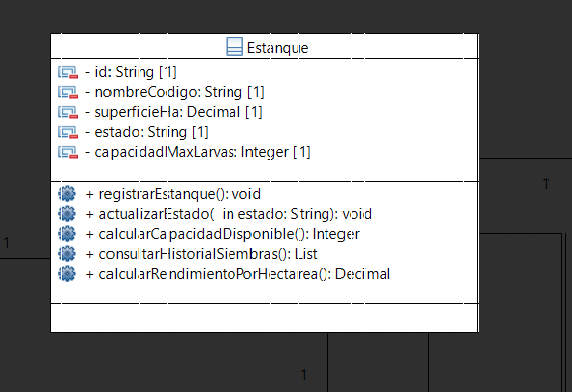
\includegraphics[width=\textwidth,keepaspectratio]{figuras/modelo_antes_cambio.png}
        \caption{Modelo antes del cambio}
        \label{fig:modelo_antes_cambio}
    \end{minipage}\hfill
    \begin{minipage}{0.48\textwidth}
        \centering
        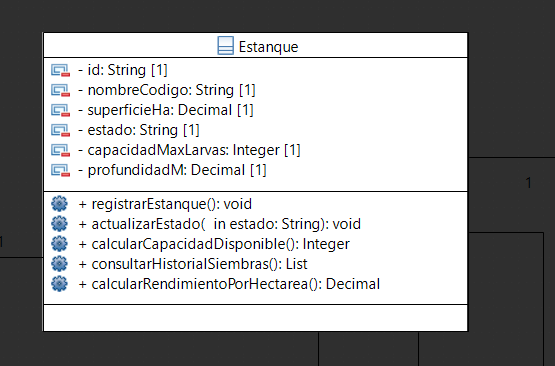
\includegraphics[width=\textwidth,keepaspectratio]{figuras/modelo_despues_cambio.png}
        \caption{Modelo después del cambio}
        \label{fig:modelo_despues_cambio}
    \end{minipage}
\end{figure}

\begin{figure}[H]
    \centering
    \begin{minipage}{0.48\textwidth}
        \centering
        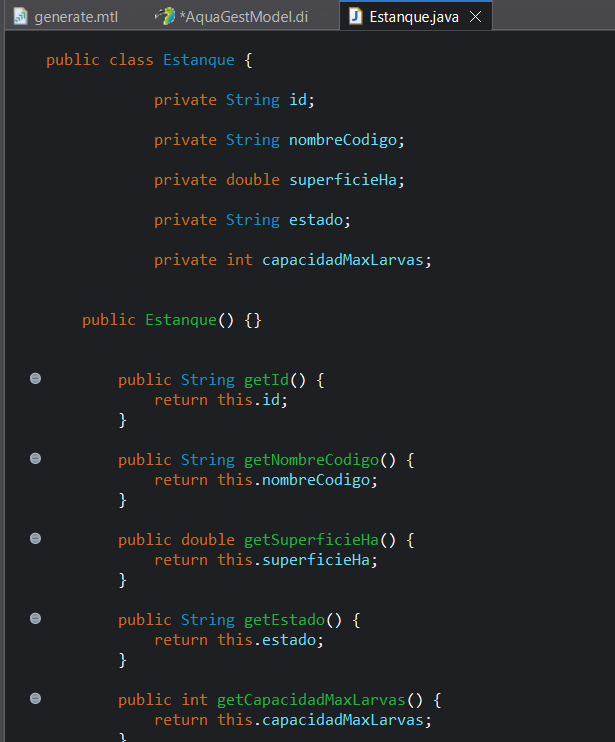
\includegraphics[width=\textwidth,keepaspectratio]{figuras/codigo_antes_regeneracion.png}
        \caption{Código antes de la regeneración}
        \label{fig:codigo_antes_regeneracion}
    \end{minipage}\hfill
    \begin{minipage}{0.48\textwidth}
        \centering
        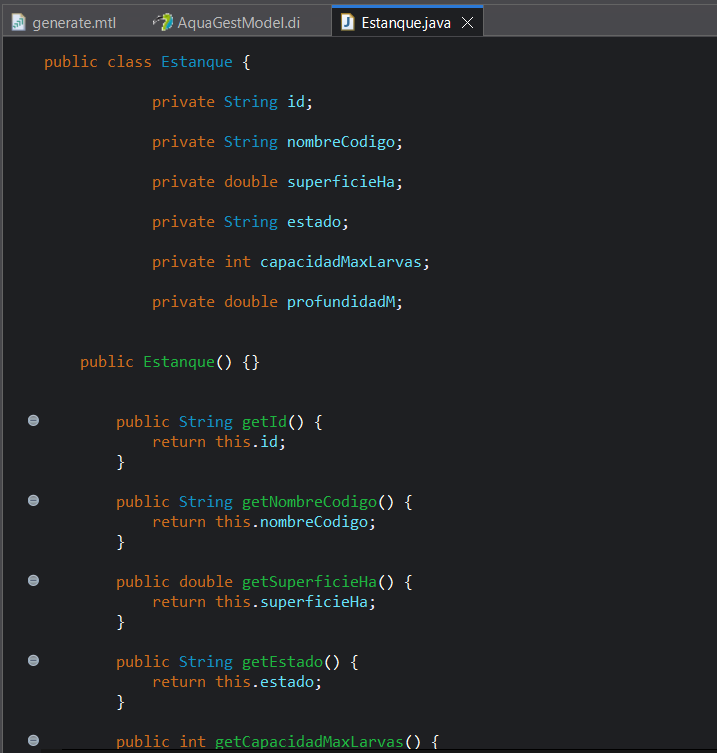
\includegraphics[width=\textwidth,keepaspectratio]{figuras/codigo_despues_regeneracion.png}
        \caption{Código después de la regeneración}
        \label{fig:codigo_despues_regeneracion}
    \end{minipage}
\end{figure}

\section{Reparto del trabajo por integrante}

La siguiente tabla documenta la distribución de responsabilidades del equipo sobre las fases del ciclo
MDD aplicado a AquaGest. Los nombres, tareas concretas y enlaces a los commits atribuibles a cada
integrante quedan pendientes de completar con la información real del equipo una vez ejecutado el
trabajo.

\begin{table}[h!]
\centering
\small
\begin{tabular}{@{}L{3cm}L{4.5cm}L{4.5cm}@{}}
\toprule
\textbf{Integrante} & \textbf{Fase(s) liderada(s)} & \textbf{Tareas concretas} \\
\midrule
Ponce Espinoza Mery Helenmay & Modelado UML & Construcción del diagrama de clases en Eclipse Papyrus, definición del perfil UML y aplicación de estereotipos sobre las clases del subsistema. \\
Pérez Ruiz Carlos Andres & Configuración del generador (Acceleo) & Adaptación del módulo \texttt{generate.mtl}, definición de las plantillas de generación de atributos, \textit{getters/setters} y métodos. \\
Gamarra Araujo Edhu Xavier & Verificación y roundtrip & Compilación del proyecto generado, ejecución de la prueba de cambio sobre el modelo y verificación de la preservación del código en bloques protegidos. \\
Sanchez Centeno Roselyn Andreina & Documento evidencia y coordinación de la exposición & Redacción del documento de evidencia, recopilación de capturas del proceso y coordinación de la entrega en el repositorio de GitHub. \\
\bottomrule
\end{tabular}
\caption{Distribución de responsabilidades por integrante (estructura a completar).}
\end{table}

\section{Conclusiones}

La aplicación planificada del ciclo MDD sobre el subsistema de gestión de alimentación y control de
estanques de AquaGest permite anticipar las siguientes conclusiones, que deberán contrastarse y
completarse con los resultados reales obtenidos tras ejecutar la demostración:

\begin{itemize}[nosep]
  \item El uso de Eclipse Papyrus junto con Acceleo, motor de transformación M2T basado en el
        estándar OMG MOFM2T, fundamenta la generación de código de AquaGest en un mecanismo
        abierto y auditable, en contraste con generadores propietarios de caja cerrada.
  \item El valor real de MDD para el PFC reside en reducir el esfuerzo de escritura manual de las
        clases de entidad del dominio y en mantener la trazabilidad explícita entre el modelo
        conceptual del negocio acuícola y el código fuente resultante.
  \item El mecanismo de bloques de código protegido de Acceleo es central para sostener un flujo de
        trabajo iterativo, en el que el modelo evoluciona sin destruir la lógica de negocio
        implementada manualmente.
  \item Como limitación y aprendizaje, se anticipa la necesidad de completar a mano la lógica no
        representable en el diagrama de clases, y se espera evidenciar en la práctica la diferencia
        entre un modelo UML documental y uno usado como artefacto de primera clase que conduce el
        desarrollo, en línea con los fundamentos de MDE del marco teórico.
\end{itemize}


\newpage
\bibliographystyle{ieeetr}
\bibliography{referencias}

\end{document}
